\documentclass[10pt,a4paper]{article}
\usepackage[latin1]{inputenc}
\usepackage{amsmath}
\usepackage{amsfonts}
\usepackage{amssymb}
\usepackage{graphicx}
\usepackage{longtable}
\usepackage{float}
\usepackage{physics}
\usepackage{soul}
\usepackage{caption}
\usepackage{subcaption}
\usepackage[section]{placeins}
\usepackage[left=2cm,right=2cm,top=2cm,bottom=2cm]{geometry}
\author{Akshat Mahajan}
\title{Physics 180Q - CHSH Inequality}
\begin{document}
\maketitle
\noindent \textsl{This lab was performed in conjunction with Hanwen Qin. The details of this experiment were spread over two consecutive lab sections.}
\section*{The Goal}
The goal of this experiment was to conclusively demonstrate the entanglement of photon pairs produced from an SPDC crystal, and then to violate the CHSH inequality, a form of Bell's inequality, using these entangled photons. To do this, we made use of the standard quED apparatus from the Qutools corporation, which consisted of a spontaneous parametric down-conversion (SPDC) crystal, a blue ($\lambda = 403$ nm) laser beam, beam-shaping optical components including a set of compensation crystals, two rotatable polarisers, and two photon detectors capable of making single-photon measurements and (jointly) measurement counts.
\section*{Part 1: Verifying Entanglement}
In theory, our blue laser beam would be converted into two red laser beams, each manipulated so as to venture off in different directions. Each individual beam would go through a polariser and then a detector. The polarisers are rotatable, enabling us to selectively filter out photon pairs. In particular, if we denote by $\ket{H_{i}}$ the horizontal polarisation state for arm $i$, and $\ket{V_{i}}$ similarly but for vertical polarisation states, we find that the total wave function for our two photons could be written out as

$$\ket{\Psi} = c_{1}\ket{H_{1}}\ket{V_{2}} + c_{2}\ket{V_{1}}\ket{H_{2}} + c_{3}\ket{H_{1}}\ket{H_{2}} + c_{4}\ket{V_{1}}\ket{V_{2}}$$

\noindent i.e. that those are all the possible measurements we could make. In practice, however, we find that the coefficients $c_{3}$ and $c_{4}$ vanish, and that there is an additional phase factor to account for, so that our actual (normalised) wave function is 

$$\ket{\Psi} = \dfrac{1}{\sqrt{2}}\left(\ket{H_{1}}\ket{V_{2}} + e^{i\phi}\ket{V_{1}}\ket{H_{2}}\right)$$

\noindent This behaviour arises in our experiment owing to the nature of the beam-shaping process - in particular, we use a nonlinear crystal and two pinholes to only allow photon pairs to pass through that are either horizontal or vertically aligned, but not both horizontal or vertical simultaneously. The phase factor $e^{i\phi}$ can be tuned by inserting a compensation crystal - a crystal whose orientation is directly correlated with $\phi$ - in one arm of the beam. Depending on the orientation of this crystal, we can prepare either of the following two states:
$$\ket{\Psi_{+}} = \dfrac{1}{\sqrt{2}}\left(\ket{H_{1}}\ket{V_{2}}+ \ket{V_{1}}\ket{H_{2}}\right)$$
$$\ket{\Psi_{-}} = \dfrac{1}{\sqrt{2}}\left(\ket{H_{1}}\ket{V_{2}} - \ket{V_{1}}\ket{H_{2}}\right)$$
(we could also prepare all states in between, but the results are clearest this way).\\
\\
Thus far, we have referred to $\ket{H_{i}}$ and $\ket{V_{i}}$ for pure  vertically and horizontally polarised states, but haven't referred to what might happen as we rotate the polarisers by some angle $\alpha$, $\beta$ respectively. It turns out that the behaviour of $\ket{\Psi_{+}}$ and $\ket{\Psi_{-}}$ differ drastically when the polarisers are rotated to a diagonal basis (i.e. to angles $\pm\frac{\pi}{4}$) - in particular, $\ket{\Psi_{+}}$ results in minimum coincidence count rates for the orientation $\alpha, \beta = \pm \frac{\pi}{4}, \mp \frac{\pi}{4}$, whereas a minimum is observed for $\ket{\Psi_{-}}$ in the orientation $\alpha, \beta = \pm \frac{\pi}{4}, \pm \frac{\pi}{4}$. Conversely, each state is at a maximum for the orientation where the other state is at a minimum. Derivations of these results are omitted for conciseness, but can be straightforwardly obtained by writing $\ket{\Psi}$ in a diagonal basis.\\
\\
A quick measure of the extent of entanglement can be defined by invoking the concept of \textsl{interferometric visibility} (or just visibility), where $C_{\mathrm{max}}$,$C_{\mathrm{min}}$ are the maximum and minimum coincidence count rates respectively for our chosen wave function:
$$V = \dfrac{C_{\mathrm{max}} - C_{\mathrm{min}}}{C_{\mathrm{max}} + C_{\mathrm{min}}}$$
$$\Delta V = \dfrac{1}{\left(C_{max} + C_{min}\right)^{2}}\times \sqrt{4C_{min}^{2}C_{max} + 4C_{max}^{2}C_{min}}$$
Ideally, this number should be as high as possible to consistently demonstrate entanglement. A slightly better measurement of visibility can be made by keeping one polariser fixed at an angle $\alpha$ while rotating the other (call the angle it's at $\beta$) from 0 to 180 degrees. Then $V$ can be determined from fitting the coincidence count rates to
\begin{equation}
C = \dfrac{A}{2}\left[1 - V\sin\left(\dfrac{\beta - \beta_{c}}{P}\right)\right]
\end{equation} 
where $A,\beta_{c}, P, V$ are all to be determined by a nonlinear fit.\\
\\
\textbf{Entanglement can be demonstrated by showing that there is no basis that separates the two states}. In other words, if we continuously rotate a polarizer while keeping the other one fixed and find that there is no way to independently change the polarisation through one arm without affecting the polarisation through the other, then we will have demonstrated entanglement. Put more simply, if there  is change in the coincidence count rates as the polariser is rotated but \textit{no} change in the single-photon count rate through that polariser, we can conclude that entanglement has been demonstrated.

\subsection*{Procedure}

As a first step, we made sure that the coincidence count rate was a linear function of the power emitted. This behaviour allows us to rule out a large number of potential systematic errors that may alter our experiment. Noting that the laser power at 38 mA operating current is 20 mW and that it vanishes linearly below the threshold current of 26 mA, we treated power as a linear function of current, and varied the current to discern the behaviour of our system. A linear fit of the form 
$$\mathrm{Counts} = \left(2.14\times\mathrm{Power}\right) + 1.5$$
fits the data well. Figure 1 displays this fit graphically.

\begin{figure}[H]
\centering
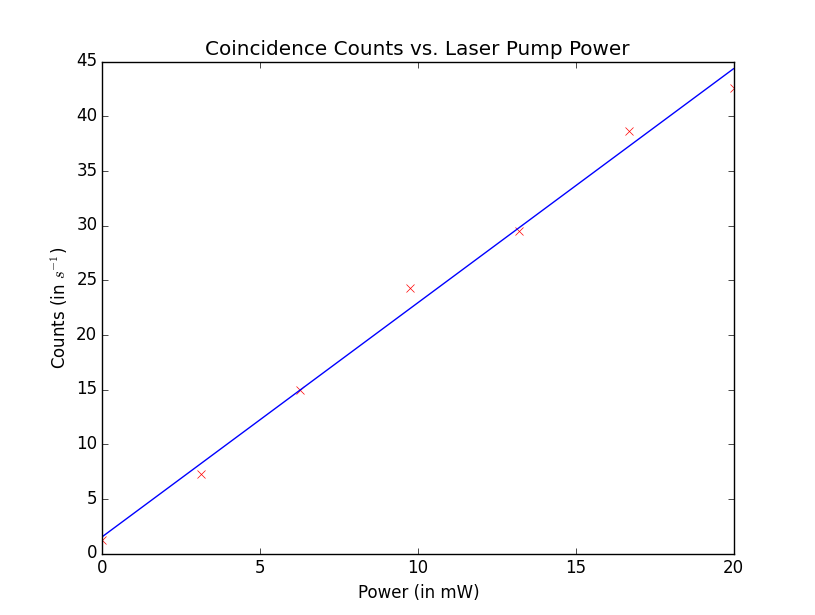
\includegraphics[scale=0.6]{../Analysis/countvspower.png}
\caption{The coincidence count rates versus laser pump power. The $R^{2}$ value for the linear fit was in excess of 99\%. The small intercept at zero power can be successfully attributed to background noise.} 
\end{figure}

\noindent We decided to discern the existing visibility of our setup, prior to any further optimisation for a chosen Bell state. We chose an integration time of 10 seconds for our detectors, and made five measurements each, of which we took the average. The horizontal and vertical transmission states of our polarisers were offset by some angles - for arm 1, the offset was 1$^{\circ}$ for the horizontal, whereas for arm 2, the angular correction in the horizontal was 7$^{\circ}$. Obviously, the vertical states were at 91$^{\circ}$ and 97$^{\circ}$ respectively.\\
\\
Table 1 contains our results for all of our optimisation attempts. Through trial and error, we found that the existing Bell state observed a maximum\footnote{By no means was either maximum or minimum optimized at the time.} at $\alpha,\beta = 45^{\circ},45^{\circ}$ (including an offset correction) and a corresponding minimum at $\alpha,\beta = 45^{\circ},-45^{\circ}$ (including an offset correction). Table 1(a) describes our results, and we compute a visibility of 73\% initially.\\
\\
We chose to optimise for the state $\ket{\Psi_{+}}$. To do this, we rotated into the diagonal basis where $\ket{\Psi_{+}}$ is a minimum, and attempted to reduce the coincidence count rate still further by altering the compensation crystal (and hence the phase). Table 1(b), 1(c) and 1(d)  document two separate efforts in this regard. We find our visibility improves to 77\% and then to 90\% respectively.
\begin{table}[H]
\centering
\begin{tabular}{|c|c|}
\hline
\multicolumn{2}{|c|}{Pre-Optimisation}\\
$C_{max}$ (s$^{-1}$) & $C_{min}$ (s$^{-1}$)\\
\hline
17.1 & 2.4 \\
19.1 & 3.1 \\
17.4 & 2.8 \\
18.7 & 2.7 \\
18.6 & 3.1 \\
\hline
\multicolumn{2}{|c|}{}\\[-2mm]
\multicolumn{2}{|c|}{$\overline{C_{max}} = 18.18$}\\
\multicolumn{2}{|c|}{$\overline{C_{min}} = 2.82$}\\
\multicolumn{2}{|c|}{$V = 0.73;\; \Delta V = 0.14$}\\
\hline
\end{tabular}
\begin{tabular}{|c|c|}
\hline
\multicolumn{2}{|c|}{First Attempt}\\
$C_{max}$ (s$^{-1}$) & $C_{min}$ (s$^{-1}$)\\
\hline
15 & 2.2 \\
19.5 & 1.6 \\
17.4 & 2.5 \\
16.6 & 2.6 \\
17.5 & 2.1 \\
\hline
\multicolumn{2}{|c|}{}\\[-2mm]
\multicolumn{2}{|c|}{$\overline{C_{max}} = 17.2$}\\
\multicolumn{2}{|c|}{$\overline{C_{min}} = 2.2$}\\
\multicolumn{2}{|c|}{$V = 0.77;\; \Delta V = 0.14$}\\
\hline
\end{tabular}
\begin{tabular}{|c|c|}
\hline
\multicolumn{2}{|c|}{Second Attempt}\\
$C_{max}$ (s$^{-1}$) & $C_{min}$ (s$^{-1}$)\\
\hline
18.2 & 2.7 \\
18.7 & 2.4 \\
17.8 & 2 \\
19.2 & 2.1 \\
18.7 & 1.9 \\
\hline
\multicolumn{2}{|c|}{}\\[-2mm]
\multicolumn{2}{|c|}{$\overline{C_{max}} = 18.52$}\\
\multicolumn{2}{|c|}{$\overline{C_{min}} = 2.22$}\\
\multicolumn{2}{|c|}{$V = 0.78;\; \Delta V = 0.13$}\\
\hline
\end{tabular}
\begin{tabular}{|c|c|}
\hline
\multicolumn{2}{|c|}{Third Attempt}\\
$C_{max}$ (s$^{-1}$) & $C_{min}$ (s$^{-1}$)\\
\hline
22.5 & 1.8 \\
25.5 & 1.1 \\
24.1 & 0.9 \\
24.8 & 0.9 \\
26.2 & 1.9 \\
\hline
\multicolumn{2}{|c|}{}\\[-2mm]
\multicolumn{2}{|c|}{$\overline{C_{max}} = 24.62$}\\
\multicolumn{2}{|c|}{$\overline{C_{min}} = 1.32$}\\
\multicolumn{2}{|c|}{$V = 0.90;\; \Delta V = 0.08$}\\
\hline
\end{tabular}
\caption{(left to right) Table 1(a), 1(b), 1(c) and 1(d)}
\end{table}
\subsection*{Demonstration of Entanglement}
\noindent To demonstrate entanglement, we chose to make two measurements: first, keeping $\alpha = 0^{\circ}$, we rotated $\beta$ from 0 to 180 degrees while recording the single-photon count through arm 2 and the coincidence count rate; then we repeated the experiment but with $\alpha = 45^{\circ}$. We initially performed our first measurements while having a visibility of only 78 $\pm$ 13 \%, but performed the second one with a visibility of 90 $\pm$ 8 \%. Both measurements together demonstrate entanglement reasonably well. Figure 2 illustrates the behaviour of the coincidence counts as a function of $\beta$ at two different fixed $\alpha$, and also demonstrates the lack of dependence of the single-photon count rates through arm 2 on $\beta$. We conclude that \textbf{entanglement has been demonstrated}.
\begin{table}[H]
\centering
\begin{tabular}{|c|c|c|c|c|}
\hline
& \multicolumn{4}{|c|}{Parameters of Best Fit}\\
& $\lvert V \rvert$ & $\beta_{c}$ & A & P\\
\hline
$\alpha = 0$ & 0.90 & 45.3 & 20  & 0.49\\
$\alpha = 45$ & 0.84 & - 0.63 & 25 & 0.50\\
\hline
\end{tabular}
\caption{Parameters of the Fit}
\end{table}
\noindent Interestingly, it appears that our `quick' measure of visibility appears to be inversely related to the more precise fit. Our 78\% visibility turns out to have had a visibility of 90\%; our 90\% visibility had a visibility of 84\%!
\begin{figure}[H]
\centering
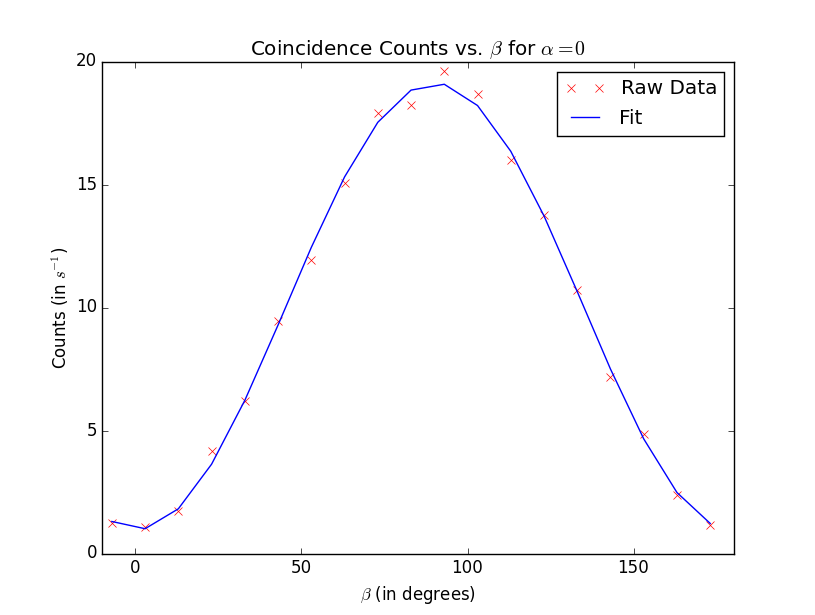
\includegraphics[scale=0.4]{../Analysis/alpha=0coinc.png}
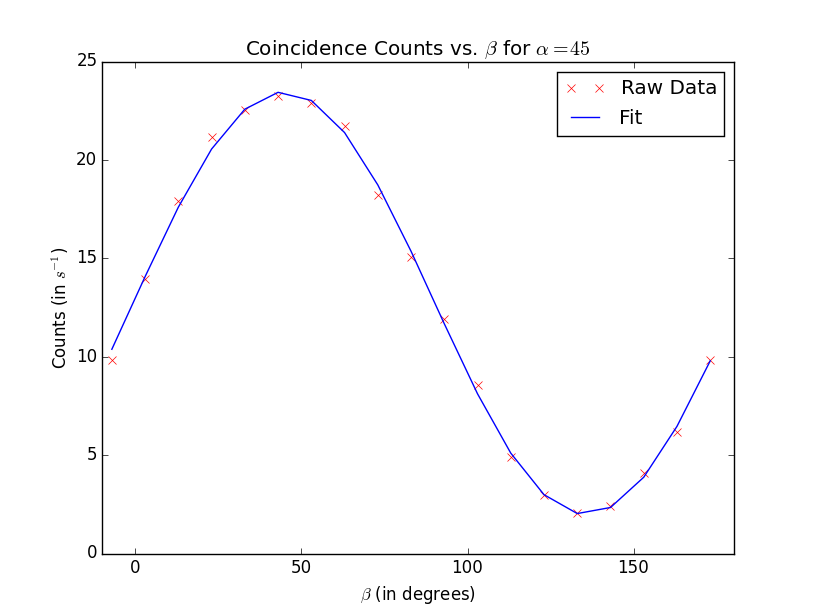
\includegraphics[scale=0.4]{../Analysis/alpha=45coinc.png}
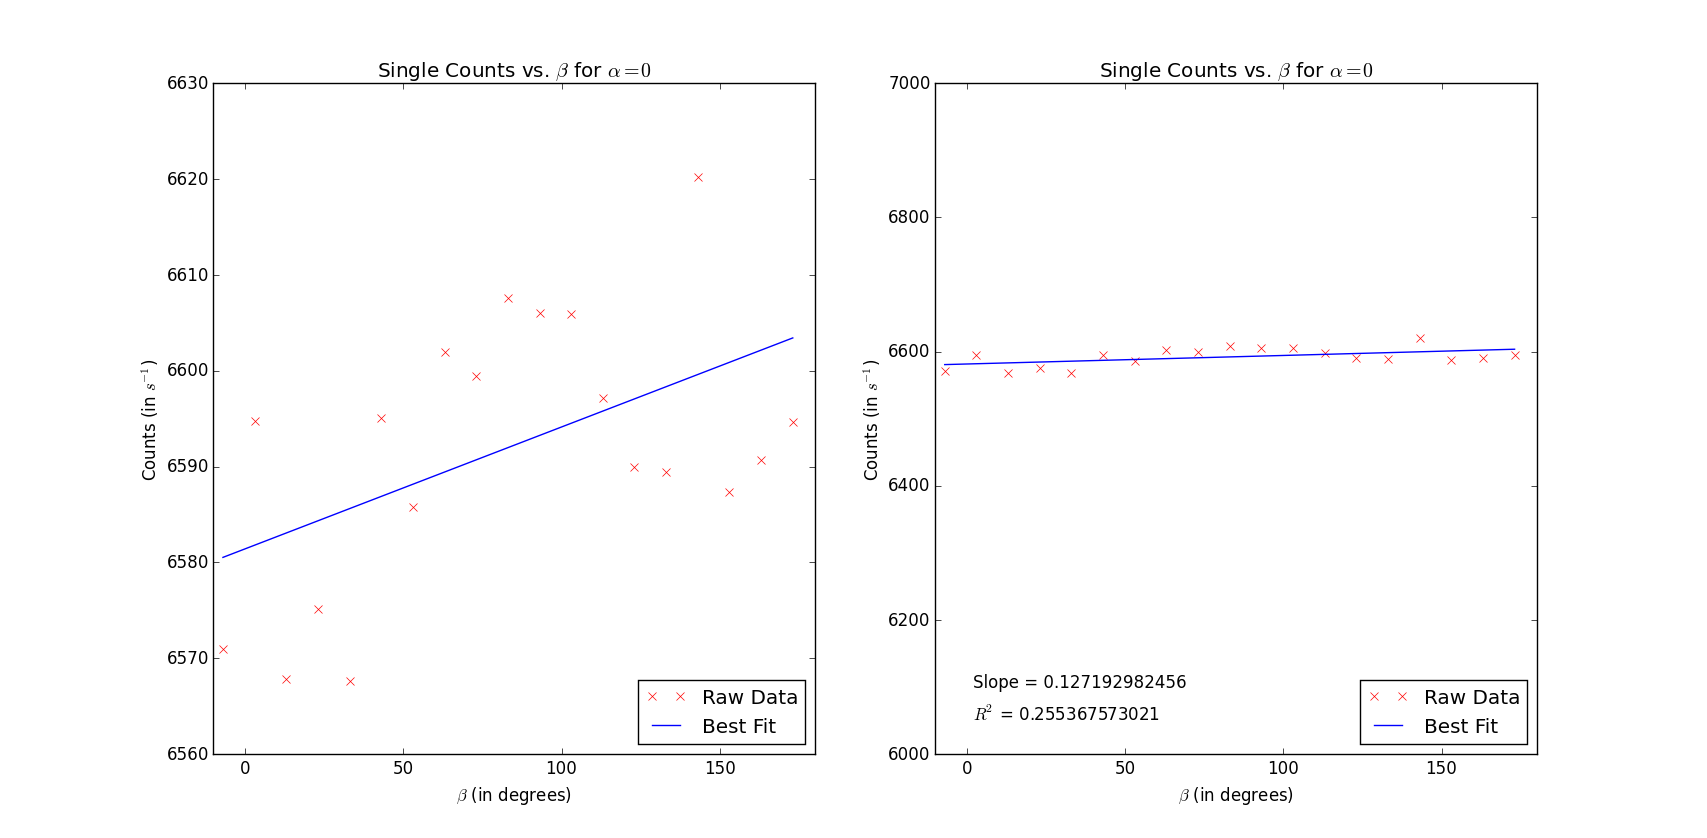
\includegraphics[scale=0.42]{../Analysis/alpha=0single.png}
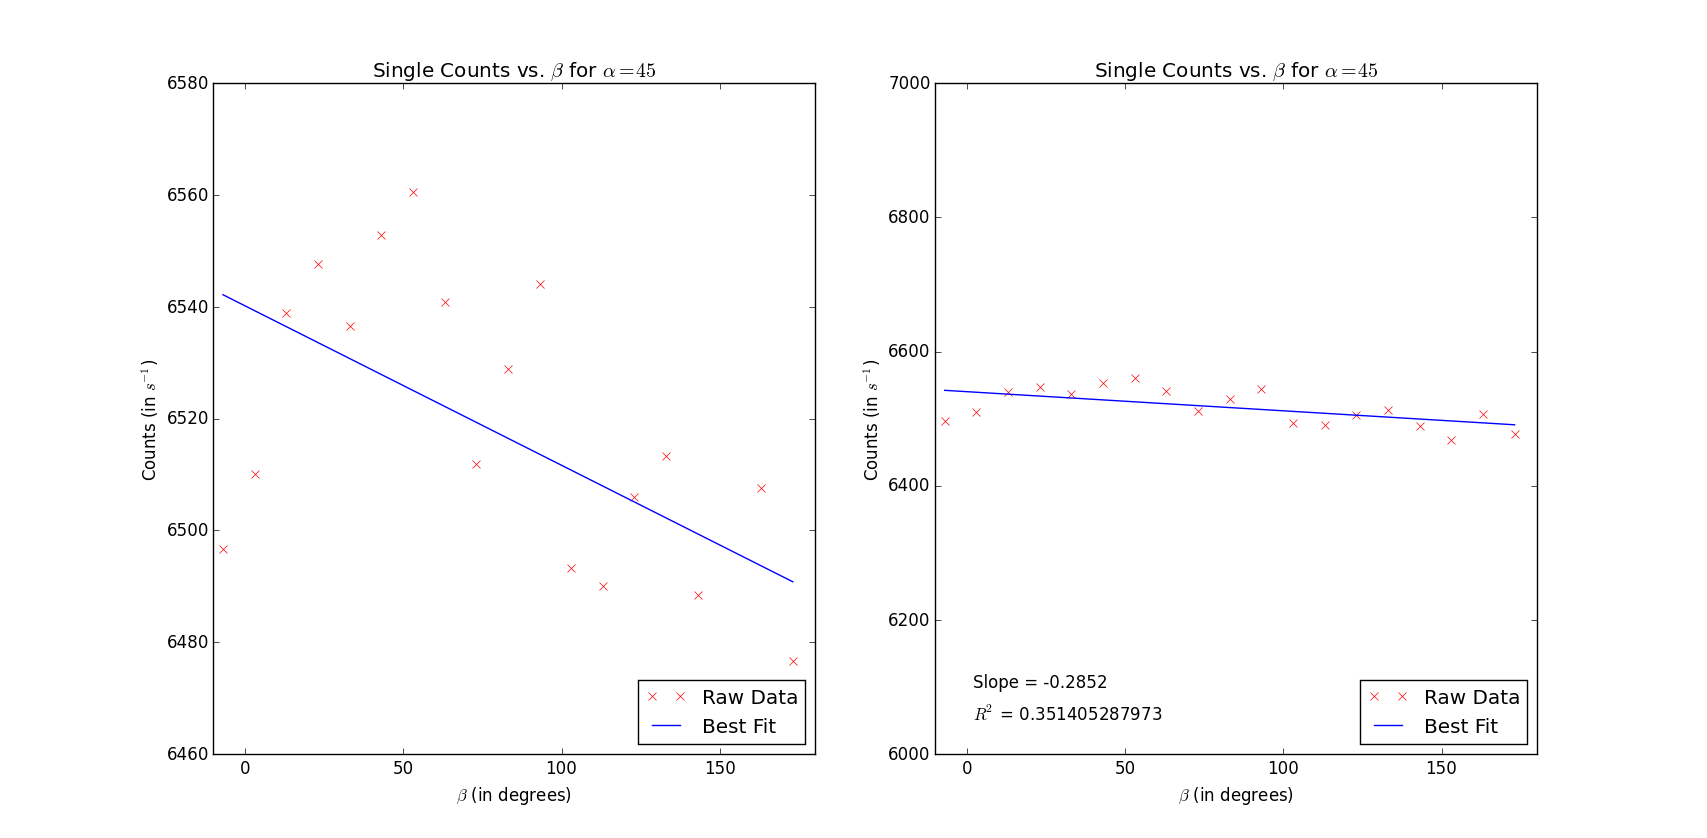
\includegraphics[scale=0.42]{../Analysis/alpha=45single.png}
\caption{Proof of entanglement. For single counts, figures on the left represent a zoomed-out version of the right. Low $R^{2}$ values indicate a random scattering of single photon count rates. Coincidence counts were fit to Equation (1).}
\end{figure}
\section*{Part 2: Violating the CHSH Inequality}
The CHSH inequality states that, if we define the following quantities\footnote{where $P_{VV}, P_{HH}$, etc. are the probabilities of observing polarisation states correspondng to the subscripts - V for vertical, H for horizontal; subscript index corresponds to arm.} for angles $\alpha,\beta,\alpha',\beta'$
$$ E(\alpha,\beta) = P_{VV}(\alpha,\beta) + P_{HH}(\alpha,\beta) - P_{HV}(\alpha,\beta) - P_{VH}(\alpha,\beta)$$
$$ S = E(\alpha,\beta) - E(\alpha,\beta') + E(\alpha',\beta) + E(\alpha',\beta')$$
then all local hidden variable theories are constrained to have $\lvert S \rvert < 2$ always. On the other hand, it is possible for quantum mechanics to have $\lvert S \rvert \geq 2$. Thus, if we observe $\lvert S \rvert \geq 2$, we will have violated the CHSH inequality and thus have shown that quantum mechanics cannot be described by a local hidden variable theory.\\
\\
In practice, we compute $E(\alpha,\beta)$ in terms of the number of coincidence counts $N$ as follows:
$$E(\alpha,\beta) = \dfrac{N(\alpha,\beta) + N(\alpha_{\bot},\beta_{\bot}) - N(\alpha_{\bot},\beta) - N(\alpha,\beta_{\bot})}{N(\alpha,\beta) + N(\alpha_{\bot},\beta_{\bot}) + N(\alpha_{\bot},\beta) + N(\alpha,\beta_{\bot})} $$ 
where the $\bot$ signs indicate rotation by 90 degrees from that angle. Furthermore, we can compute the uncertainty in $S$ as follows:
$$ \Delta S = \sqrt{\Delta E(a,b)^{2} + \Delta E(a',b)^{2} + \Delta E(a,b')^{2} + \Delta E(a',b')^{2}} $$
where 
$$ \Delta E = 2 \sqrt{\dfrac{\left[N(a,b) + N(a_{\bot},b_{\bot})\right]\left[N(a,b_{\bot}) + N(a_{\bot},b)\right]}{\left(N(a,b) + N(a_{\bot},b_{\bot}) + N(a_{\bot},b) + N(a,b_{\bot})\right)^{3}}}$$
We chose $\alpha,\beta,\alpha',\beta' = -45^{\circ},-22.5^{\circ},0^{\circ},22.5^{\circ}$ \textbf{for\footnote{We are entirely free to choose any set of angles we want to test Bell's inequality against. Using different angles for different states does not alter the validity of our conclusion - it only changes which quantity we apply our negative sign to for $S$. Explicit calculations below should reveal this more carefully.} the state $\ket{\Psi_{-}}$} and $\alpha,\beta,\alpha',\beta' = -45^{\circ},22.5^{\circ},0^{\circ},-22.5^{\circ}$ \textbf{for the state $\ket{\Psi_{+}}$}. We kept all arises fully open, and took five measurements at ten seconds each for every measurement. Here, we report only the average values of our results for brevity. We prepared both $\ket{\Psi_{+}}$ and $\ket{\Psi_{-}}$ states, and observed a violation of the CHSH inequality for both.
\subsection*{For $\ket{\Psi_{+}}$ State}
Table 3 describes our attempts to optimise towards this state. All angles reported are inclusive of corrections.
\begin{table}[H]
\centering
\begin{tabular}{|c|c|}
\hline
\multicolumn{2}{|c|}{Optimisation}\\
$C_{max}$ (s$^{-1}$) & $C_{min}$ (s$^{-1}$)\\
\hline
24.3 & 1.5 \\
22.3 & 2.2 \\
20.6 & 1.8 \\
21.6 & 2.5 \\
22.1 & 2.1 \\
\hline
\multicolumn{2}{|c|}{}\\[-2mm]
\multicolumn{2}{|c|}{$\overline{C_{max}} = 22.18$}\\
\multicolumn{2}{|c|}{$\overline{C_{min}} = 2.02$}\\
\multicolumn{2}{|c|}{$V = 0.83;\; \Delta V = 0.11$}\\
\hline
\end{tabular}
\caption{Visibility checks for state $\ket{\Psi_{+}}$}
\end{table}
\begin{longtable}{|c|c|c|}
\hline
$\alpha$ & $\beta$ & Coincidence Counts (in s$^{-1}$)\\
\hline
-45 & -22.5 & 12.58\\
-45 & 22.5 & 1.48\\
-45 & 67.5 & 11.68\\
-45 & 112.5 & 23.64\\
\hline
0 & -22.5 & 3.6\\
0 & 22.5 & 3.52\\
0 & 67.5 & 19.38\\
0 & 112.5 & 19.78\\
\hline
45 & -22.5 & 4.24\\
45 & 22.5 & 15.76\\
45 & 67.5 & 17.84\\
45 & 112.5 & 4.02\\
\hline
90 & -22.5 & 14.82\\
90 & 22.5 & 15.78\\
90 & 67.5 & 3.12\\
90 & 112.5 & 3.54\\
\hline
\caption{Coincidence counts at various angle combinations}
\end{longtable}
\noindent From this, we see that
\begin{align*}
E(-45, -22.5) &= \dfrac{12.58 + 17.84 - 4.24 - 11.68}{12.58 + 11.68 + 4.24 + 17.84} = \dfrac{14.5}{46.34} &= 0.319\\
\Delta E(-45, -22.5) &= 2\sqrt{\dfrac{(12.58 + 17.84)\times(4.24 + 11.68)}{46.34^{3}}} &= 0.139\\
E(-45, 22.5) &= \dfrac{1.48 + 4.02 - 15.76 - 23.64}{1.48 + 4.02 + 15.76 + 23.64} = \dfrac{-33.9}{44.9} &= -0.755\\
\Delta E(-45, 22.5) &= 2\sqrt{\dfrac{(1.48 + 4.02)\times(15.76 + 23.64)}{44.9^{3}}} &= 0.097\\
E(0,-22.5) &= \dfrac{3.6 + 3.12 - 14.82 - 19.38}{3.6 + 3.12 + 14.82 + 19.38} = \dfrac{-27.48}{40.92} &= -0.672\\
\Delta E(0, -22.5) &= 2\sqrt{\dfrac{(3.6 + 3.12)\times(14.82 + 19.38)}{40.92^{3}}} &= 0.115\\
E(0,22.5) &= \dfrac{3.52 + 3.54 - 19.78 - 15.78}{3.52 + 3.54 + 15.78 + 3.54} = \dfrac{-28.5}{42.62} &= -0.658\\
\Delta E(0,22.5) &= 2\sqrt{\dfrac{(3.52 + 3.54)\times(19.78 + 15.78)}{42.62^{3}}} &= 0.113\\
\end{align*}
\noindent so that, since we've specified our $\beta,\beta' = 22.5^{\circ}, -22.5^{\circ}$, we have
\begin{align*}
\lvert| S \rvert| + \Delta S &= \lvert|E(-45, 22.5) - E(-45, -22.5) + E(0,-22.5) + E(0,-22.5)\rvert|\\
&\;\pm \sqrt{\Delta E(-45, -22.5)^{2} + \Delta E(-45, 22.5)^{2} + \Delta E(0,-22.5)^{2} + \Delta E(0,-22.5)^{2}}\\
&= \lvert|-0.755 - 0.319 - 0.672 - 0.658 \rvert| \pm \sqrt{0.139^{2} + 0.097^{2} + 0.115^{2} + 0.113^{2}}\\
&= 2.404 \pm 0.233
\end{align*}
\noindent violating Bell's ineqaaulity by roughly two standard deviations.
\subsection*{For $\ket{\Psi_{-}}$ State}
Table 5 describes our attempts to optimise towards this state. All angles reported are inclusive of corrections.
\begin{table}[H]
\centering
\begin{tabular}{|c|c|}
\hline
\multicolumn{2}{|c|}{Optimisation}\\
$C_{max}$ (s$^{-1}$) & $C_{min}$ (s$^{-1}$)\\
\hline
16.6 & 2.2 \\
19.2 & 3.2 \\
19.2 & 3 \\
18.2 & 2.7 \\
17.6 & 2.9 \\
\hline
\multicolumn{2}{|c|}{}\\[-2mm]
\multicolumn{2}{|c|}{$\overline{C_{max}} = 18.16$}\\
\multicolumn{2}{|c|}{$\overline{C_{min}} = 2.8$}\\
\multicolumn{2}{|c|}{$V = 0.73;\; \Delta V = 0.14$}\\
\hline
\end{tabular}
\caption{Visibility checks for state $\ket{\Psi_{-}}$}
\end{table}
\begin{longtable}{|c|c|c|}
\hline
$\alpha$ & $\beta$ & Coincidence Counts (in s$^{-1}$)\\
\hline
-45 & -22.5 & 1.8\\
-45 & 22.5 & 11.3\\
-45 & 67.5 & 21.22\\
-45 & 112.5 & 10.12\\
\hline
0 & -22.5 & 3.42\\
0 & 22.5 & 3.76\\
0 & 67.5 & 19.38\\
0 & 112.5 & 19.66\\
\hline
45 & -22.5 & 14.88\\
45 & 22.5 & 4.32\\
45 & 67.5 & 5.76\\
45 & 112.5 & 20.2\\
\hline
90 & -22.5 & 15.06\\
90 & 22.5 & 13.2\\
90 & 67.5 & 2.64\\
90 & 112.5 & 4.8\\
\hline
\caption{Coincidence counts at various angle combinations}
\end{longtable}
\noindent From this, we see that 
\begin{align*}
E(-45, -22.5) &= \dfrac{1.8 + 5.76 - 21.22 - 14.88}{1.8 + 5.76 + 21.22 + 14.88} = \dfrac{-28.54}{43.66} &= -0.654\\
\Delta E(-45, -22.5) &= 2\sqrt{\dfrac{(1.8 + 5.76)\times(21.22 + 14.88)}{43.66^{3}}} &= 0.114\\
E(-45, 22.5) &= \dfrac{11.3 + 20.2 - 10.12 - 4.32}{1.48 + 4.02 + 15.76 + 23.64} = \dfrac{17.06}{45.94} &= 0.371\\
\Delta E(-45, 22.5) &= 2\sqrt{\dfrac{(11.3 + 20.2)\times(10.12 + 4.32)}{45.94^{3}}} &= 0.136\\
E(0,-22.5) &= \dfrac{3.42 + 4.8 - 15.06 - 21.22}{3.6 + 3.12 + 14.82 + 19.38} = \dfrac{-28.06}{44.5} &= -0.630\\
\Delta E(0, -22.5) &= 2\sqrt{\dfrac{(3.42 + 4.8)\times(15.06 + 21.22)}{44.5^{3}}} &= 0.116\\
E(0,22.5) &= \dfrac{3.76 + 4.8 - 19.66 - 13.2}{3.52 + 3.54 + 15.78 + 3.54} = \dfrac{-24.3}{41.42} &= -0.586\\
\Delta E(0,22.5) &= 2\sqrt{\dfrac{(3.76 + 4.8)\times(19.66 + 13.2)}{41.42^{3}}} &= 0.125\\
\end{align*}
\noindent so that, since we've specified our $\beta,\beta' = -22.5^{\circ}, 22.5^{\circ}$, we have
\begin{align*}
\lvert| S \rvert| \pm \Delta S &= \lvert|E(-45, -22.5) - E(-45, 22.5) + E(0,-22.5) + E(0,-22.5)\rvert|\\
&\;\pm \sqrt{\Delta E(-45, -22.5)^{2} + \Delta E(-45, 22.5)^{2} + \Delta E(0,-22.5)^{2} + \Delta E(0,-22.5)^{2}}\\
&= \lvert|- 0.654 - 0.317 - 0.630 - 0.586 \rvert| \pm \sqrt{0.114^{2} + 0.136^{2} + 0.116^{2} + 0.125^{2}}\\
&= 2.187 \pm 0.246
\end{align*}
\section*{Summary}
We have successfully demonstrated entanglement as well as a violation of the CHSH inequality in both cases. While the standard deviation of $S$ for $\ket{\Psi_{-}}$ leaves some margin for error,  we were able to conclusively demonstrate a Bell's inequality violation for $\ket{\Psi_{+}}$ (for which we had the stronger visibility in any case).
\end{document}